\section{Materials}\label{sec:Materials}
\todo[inline, color=yellow]{Laura}
The following sections describe the resources and tools required for the completion of the project. Furthermore, the test images are presented in section~\ref{sec:testimages}.


\subsection{Hardware}\label{sec:Hardware}
\todo[inline, color=yellow]{Laura}
During the implementation phase, the application was run on two computers, which are described in the following two sections. Both computers needed to be able to deal with the software components described in section \ref{sec:Software}. An extract from their data sheet is shown in table \ref{tab:Computer1} respectively table \ref{tab:Computer2}.


\begin{table}
	\centering
	\begin{tabular}{|l|l|}
		\hline
		\Absatzbox{}
		\textbf{\textcolor{red}{NAME?}}& \textbf{Description} \\
		\hline
		Processor & \textcolor{red}{??} \\
		\hline
		RAM & \textcolor{red}{??}  \\
 		\hline 
		Graphic Card & \textcolor{red}{??} \\
		\hline
		Operating System & \textcolor{red}{??}  \\
		\hline
	\end{tabular}
	\caption[Extract from the Data Sheet of the \textcolor{red}{NAME?}]{Extract from the Data Sheet of the \textcolor{red}{NAME?}}.
	\label{tab:Computer1}
\end{table}

\begin{table}
	\centering
	\begin{tabular}{|l|l|}
		\hline
		\Absatzbox{}
		\textbf{Acer Aspire 5820TG}& \textbf{Description} \\
		\hline
		Processor & Intel Core i3 CPU @ $2.40\,$GHz \\
		\hline
		RAM & $4\,$GB \\
 		\hline 
		Graphic Card 1 & AMD Mobilty Radeon HD 5000 Series\\
		\hline
		Graphic Card 2 & Intel(R) HD Graphics\\
		\hline
		Operating System & Windows 10 Education 64 bit \\
		\hline
	\end{tabular}
	\caption[Extract from the Data Sheet of the Acer Aspire 5820TG Notebook.]{Extract from the Data Sheet of the Acer Aspire 5820TG Notebook.}
	\label{tab:Computer2}
\end{table}


\subsection{Software} \label{sec:Software}
\todo[inline, color=yellow]{Laura}
In order to develop the \textit{Interactive Lighting Detector} \textit{Qt} was used (compare section \ref{sec:qt}). To take advantage of already existing functionalities the \textit{OpenCV}-library, which is described in section \ref{sec:opencv}, was included in the project.


\subsubsection{QT} \label{sec:qt}
\todo[inline, color=yellow]{Laura}
The \textit{QT Creator} was invented by \textit{The Qt Company}. It is an integrated software development environment in the programming language C++. More functionality can be added by using the Qt project's library, which is called \textit{Qt}.
As a cross-platform tool, the \textit{QT Creator} can be used on all common operating systems \cite{QTCreator}. \\ Besides extensive database functions and XML-support the software can build graphic user interfaces (GUI).\\
For this project the algorithm was transcribed in source code using the \textit{Qt Creator} and the GUI was designed in the \textit{Qt Designer} \cite{website:QtDesigner}.




\subsubsection{OpenCV} \label{sec:opencv}
\todo[inline, color=yellow]{Laura}
The \textit{Open Source Computer Vision} (OpenCV) is an open source library for image- and video processing, which is among others available in the programming language \textit{C}$++$. It has been introduced ten years ago and is developed by various programmers since then. This library offers the most common algorithms, as well as current developments in image processing \cite{article:OpenCV}.\\
In the case of the implementation of the \textit{Interactive Lighting Detector} the library was mainly used for the detecting of the contours (compare section~\ref{sec:contours}) and solving the minimization problem (compare section~\ref{sec:approaches}) introduced by Johnson and Farid~\cite{Johnson}.


\subsection{Testimages} \label{sec:testimages}
\todo[inline, color=yellow]{Laura}
Due to the assumption that the objects shown on the test images described in section~\ref{sec:testimagesfirst} have a too complicated shape, a second batch of images was made (compare section~\ref{sec:testimagessecond}). Images of both batches were used to test the functionality of the the algorithms used for the lighting detection. All images have in common that besides the actual object, they show a sundial to simplify the determination of the light direction for the user.


\subsubsection{First Batch} \label{sec:testimagesfirst}
\todo[inline, color=yellow]{Laura}
Four examples of the first batch of test images are shown in figure \ref{fig:batch1}. Next to the mandatory sundial there are different objects depicted, like a helmet, a handbag, a bucket or a hot-water bottle. Those objects differ in their surface texture, as well as their size. They are shot from different angles to produce different light directions. It is necessary that the objects are not trimmed at the boarders of the image, because the algorithm requires a full contour of the selected object.


\begin{figure}[H] 
	\center 
	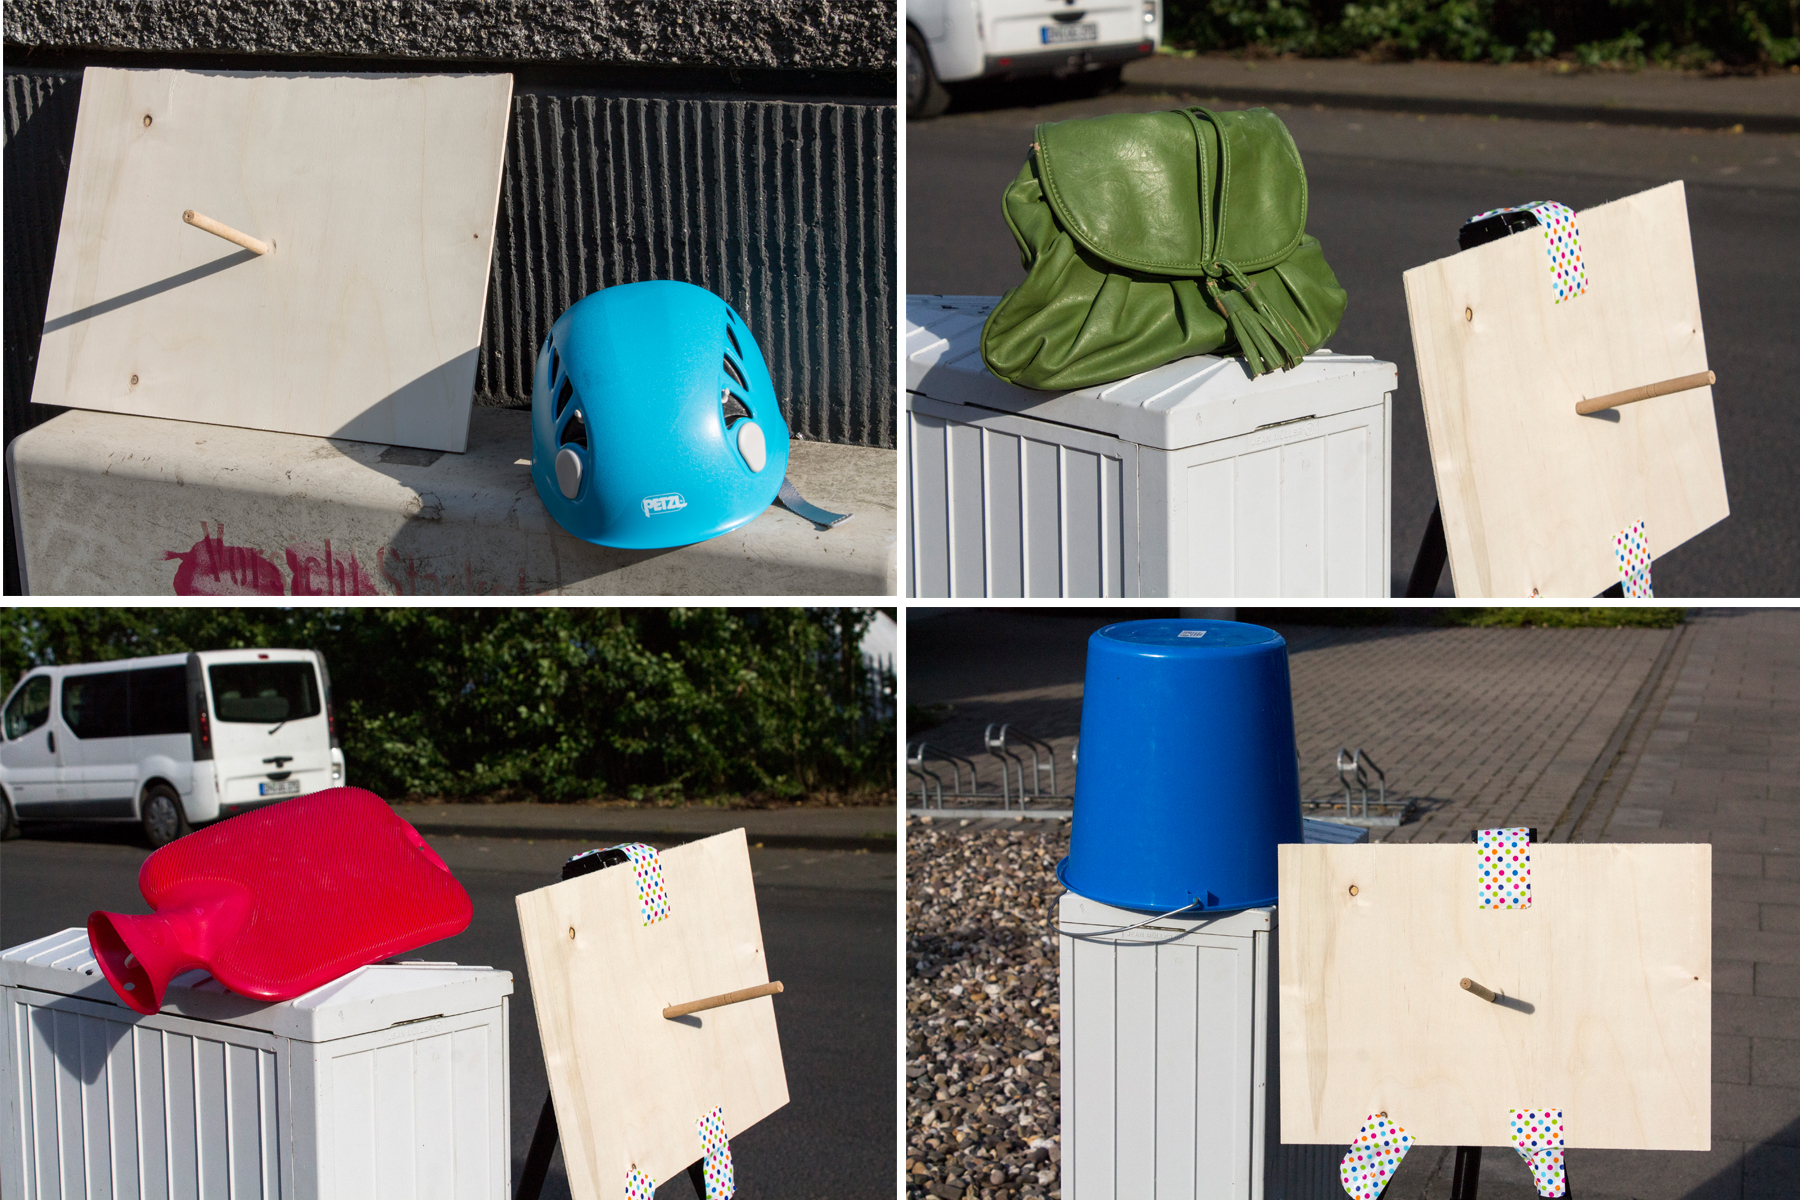
\includegraphics[width=12cm]{Images/batch1.jpg}			
	\caption[Examples of the Test Images of the first Batch.]{Examples of the Test Images of the first Batch.}
	\label{fig:batch1}
\end{figure}

\subsubsection{Second Batch} \label{sec:testimagessecond}
\todo[inline, color=yellow]{Laura}
In contrast to the first batch, the test images described in this section show easier objects with a round surface. As depicted in figure \ref{fig:batch2} all images show the madatory sundial and one or two table tennis balls in yellow and pink, which have a matt texture. For the actual algorithm of the \textit{Interactive Lighting Detector} only one of this balls is taken into consideration (compare section~\ref{sec:System}). Properties like size of the object, the camera angle and the lighting direction differs in each image.

\begin{figure}[H] 
	\center 
	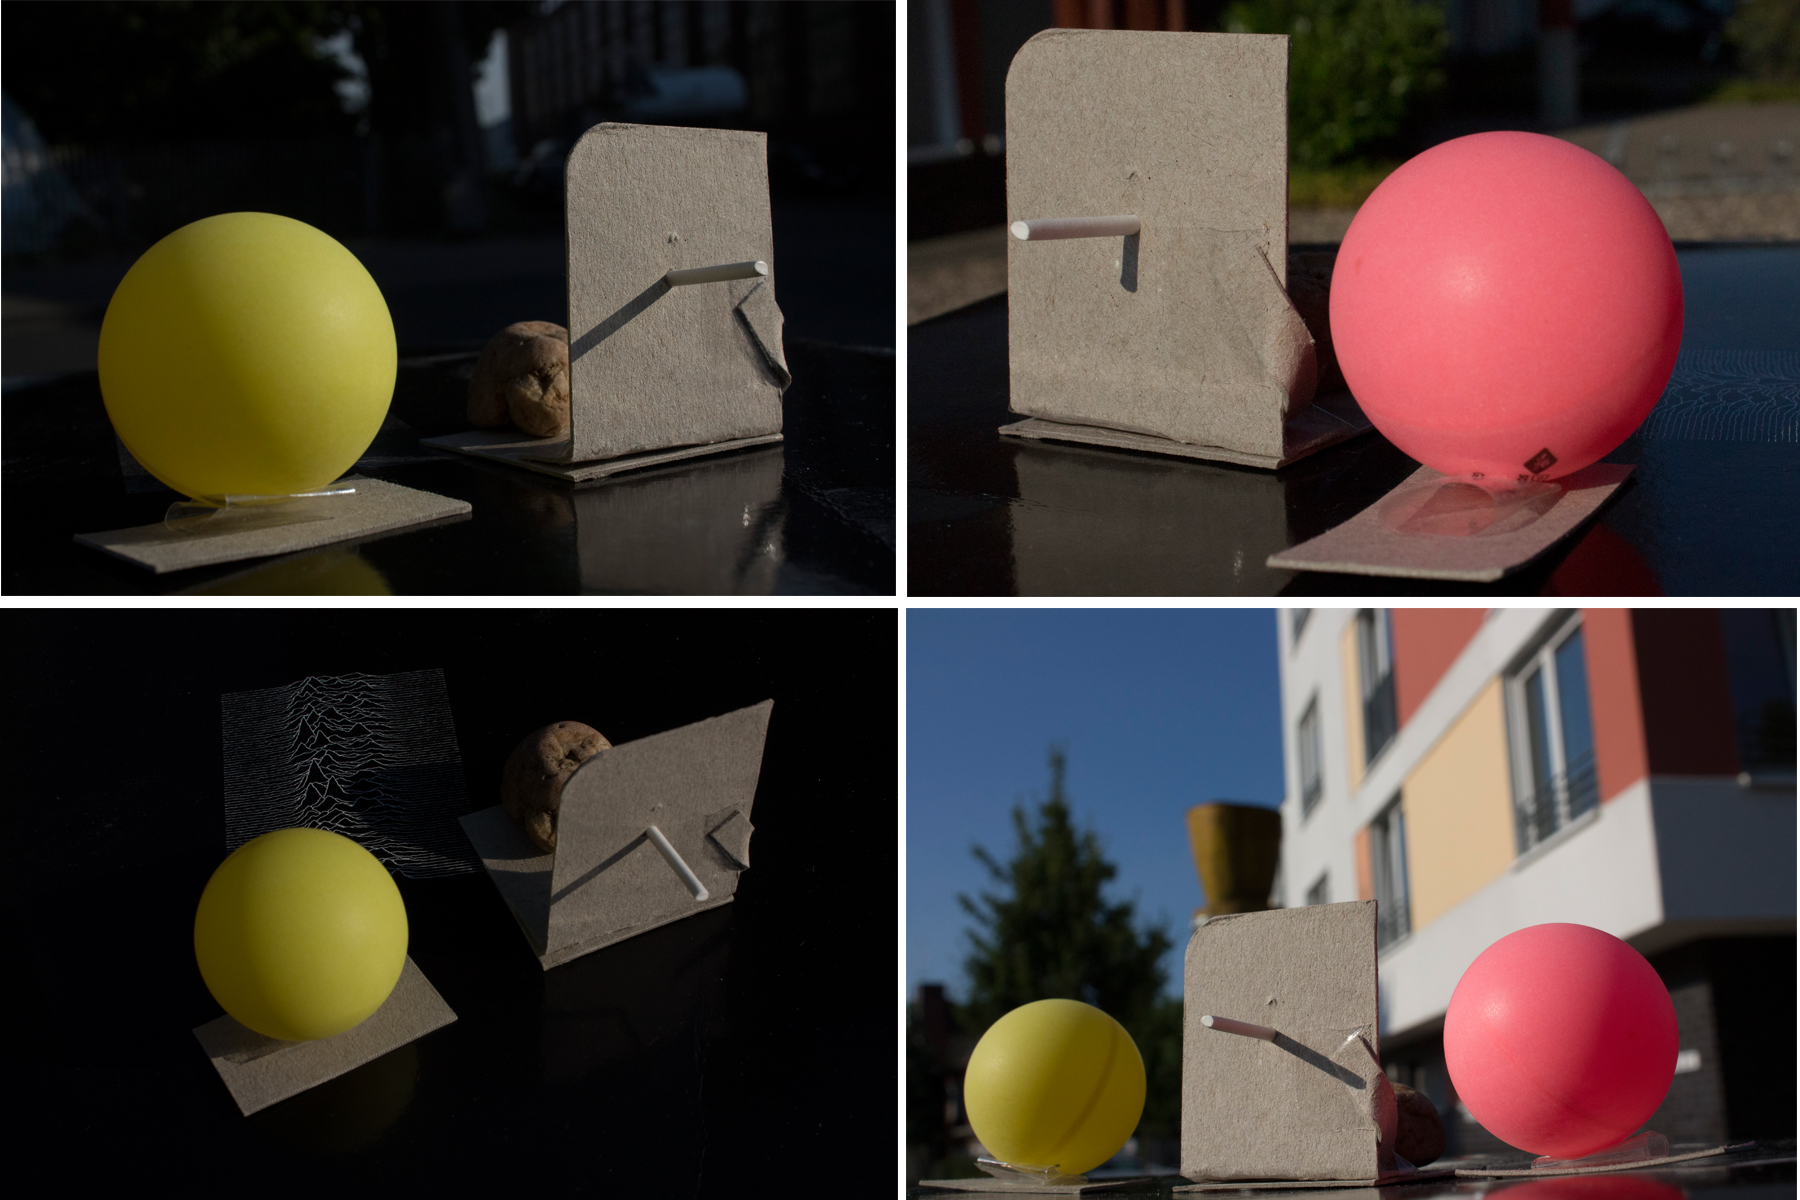
\includegraphics[width=12cm]{Images/batch2.jpg}			
	\caption[Examples of the Test Images of the second Batch.]{Examples of the Test Images of the second Batch.}
	\label{fig:batch2}
\end{figure}

\newpage